\documentclass[../main.tex]{subfiles}

\begin{document}

    \subsubsection{Model maszyny stanowej}

    \begin{figure}[H]
        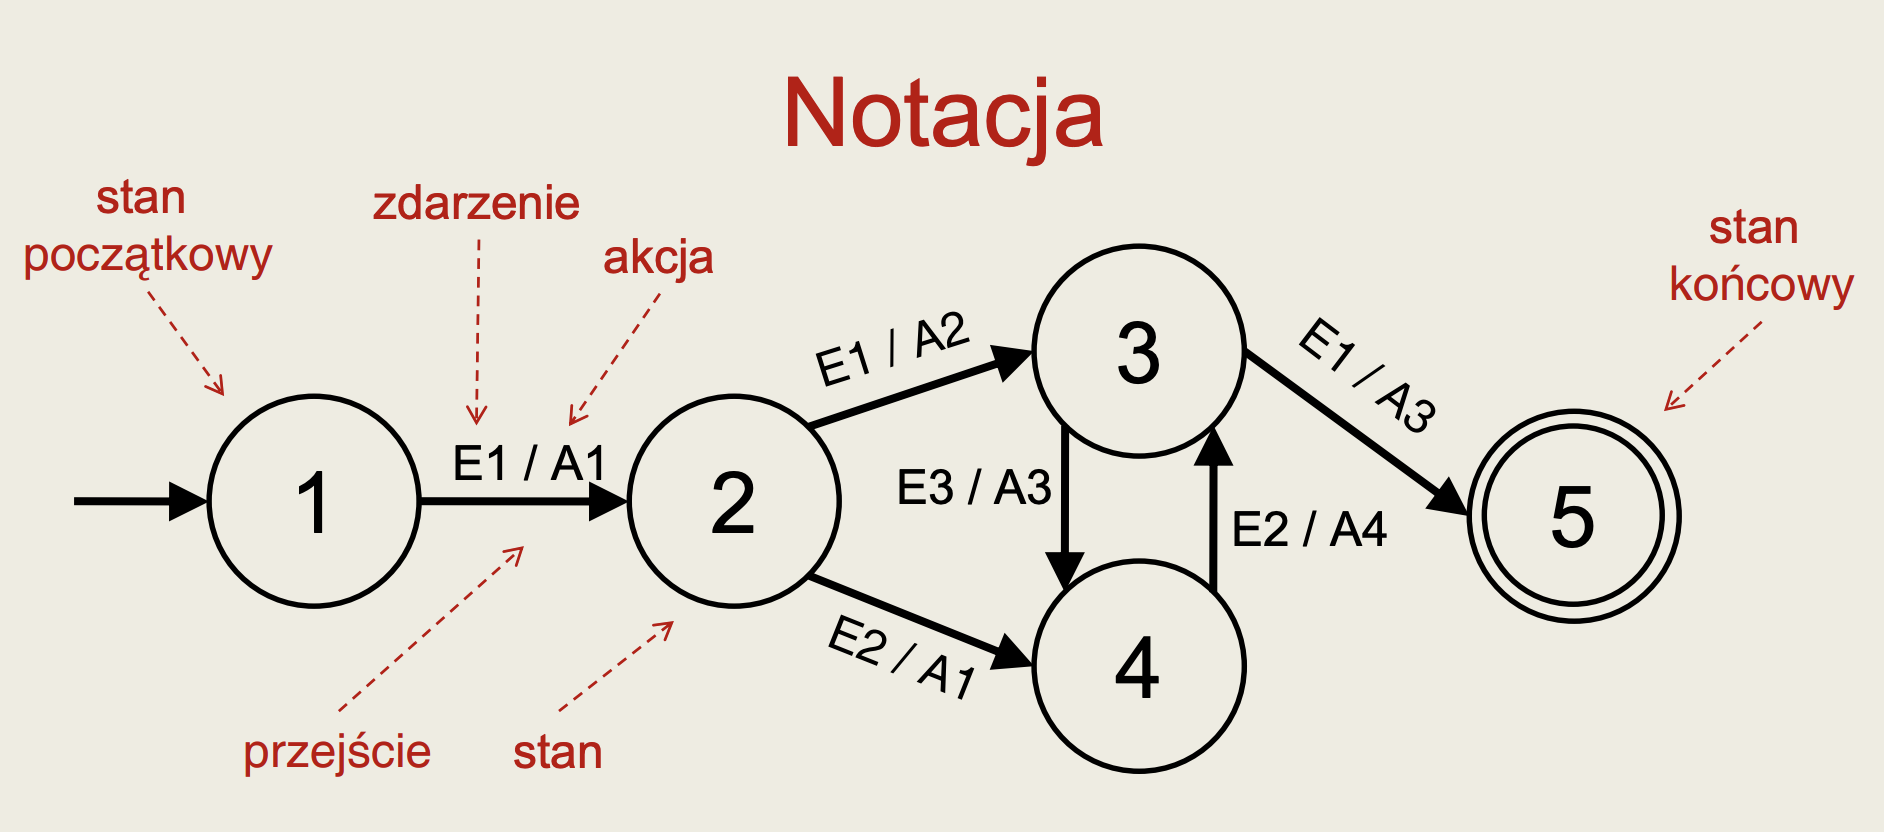
\includegraphics[width=\linewidth]{maszyna.png}
    \end{figure}

    \textbf{Tablica przejść} deifniuje akcje i przejścia dla wszystkich kombinacji stan/zdarzenie.

    \textbf{Testowanie maszyny stanowej}
    \begin{itemize}
        \item reprezentacja możliwych stanów systemu i przejść między nimi
        \item metoda opisu dynamiki systemu
        \item testowanie może sprawdzać np.:
        \begin{itemize}
            \item czy wszystkie przejścia są poprawne?
            \item czy określone sekwencje przejść są poprawne?
            \item czy da się wymusić przejścia niepoprawne?
        \end{itemize}
        \item model maszyny stanowej jest jednym z najpopularniejszych modeli
        opisu systemu
        \item UML: state chart diagram
        \begin{itemize}
            \item znacznie bogatszy niż model opisywany w niniejszym wykładzie!
        \end{itemize}
    \end{itemize}

    \textbf{n-switch coverage} - pokrycie przejść o \textbf{n} stanach pomiędzy stanem początkowym i końcowym.
    Żeby zidentyfikować pokrycie n-switchy zidentyfikuj wszystkie (n-1)-switche i ich rozszerzenia.

    \subsubsection{Drzewa klasyfikacji}
    \begin{itemize}
        \item nie mylić z modelem nauczania maszynowego!
        \item szczególna wersja metody Category-Partition
        \item graficzna reprezentacja systemu jako:
        \begin{itemize}
            \item zestawu cech
            \item ich wartości (tworzących dla każdej cechy poprawny podział)
            \item ewentualnych związków między wartościami cech
        \end{itemize}
        \item odmiana metody: model cech (ang. feature model)
        \item wykorzystywany jako model w podejściu SPL (Software Product Lines)
        \item wyprowadzanie testów wykorzystuje zwykle jedno z podejść
        kombinacyjnych
    \end{itemize}

    \begin{figure}[H]
        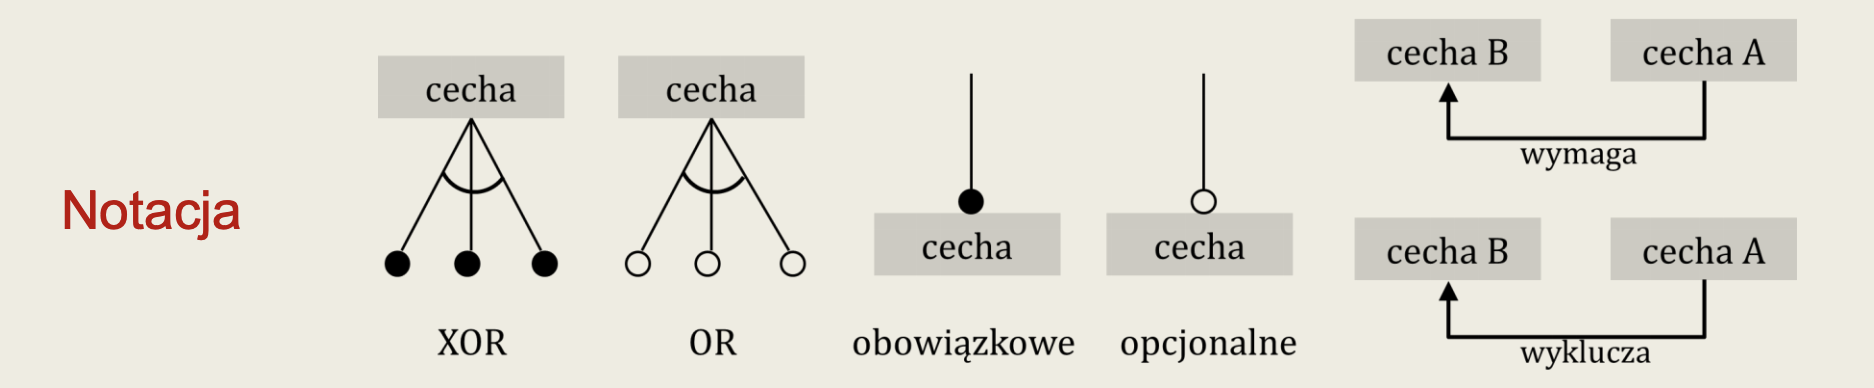
\includegraphics[width=\linewidth]{drzewa.png}
    \end{figure}

    \subsubsection{Testowanie kombinatoryczne}
    \begin{itemize}
        \item stosowane gdy chcemy testować kombinacje klas równoważności
        różnych podziałów
        \item strategia „każdy z każdym” prowadzi do eksplozji kombinatorycznej
        \item metody kombinatoryczne pozwalają na redukcję liczby testów
        \item redukcja liczby testów jest nieodłącznie związana z ryzykiem!
    \end{itemize}

    \textbf{Pełne pokrycie kombinatoryczne} = każda kombinacja klas wszystkich podziałów.

    \textbf{1-wise, Each Choice} = każda klasa z każdego podziału ma być przetestowana przynajmniej raz.
    Liczba kombinacji = max ilości klas.

    \textbf{2-wise, Pairwise} = każda para klas z dowolnych dwóch podziałów musi wystąpić przynajmniej raz. Minimalna
    liczba kombinacji jest NP-zupełna.


    \subsubsection{Testowanie losowe}
    \begin{itemize}
        \item wymaga możliwości losowego wyboru elementu dziedziny
        \item może być przeprowadzane manualnie, ale zwykle automatyczne
        \item zwykle mniej efektywne niż ine metody
        \item można stosować, gdy trudno modelować dziedzinę wejściową
        \item testowanie losowe może wykorzystywać
        \begin{itemize}
            \item rozkłady prawdopodobieństwa uwzględniające np. typowe
            zachowania użytkowników
            \item modele losowości, np. łańcuchy Markowa
        \end{itemize}
    \end{itemize}

    \textbf{Automatyzacja testowania losowego}.

    Pełna automatyzacja testowania losowego jest możliwa gdy:
    \begin{itemize}
        \item można automatyczne losować dane wejściowe
        \item można automatycznie określać oczekiwane wyjście lub automatycznie porównywać wyjście ze specyfikacją
    \end{itemize}

    To ostatnie możliwe, gdy:
    \begin{itemize}
        \item istnieje wyrocznia (np. zewnętrzny, redundantny system)
        \item interesuje nas tylko to, czy wykonanie zakończy się crashem
        \item natura wyjścia sprawia łatwość weryfikacji (np. sortowanie)
        \item łatwo wygenerować wejście z wyjścia (np. pierwiastek/potęga)
    \end{itemize}

    \begin{figure}[H]
        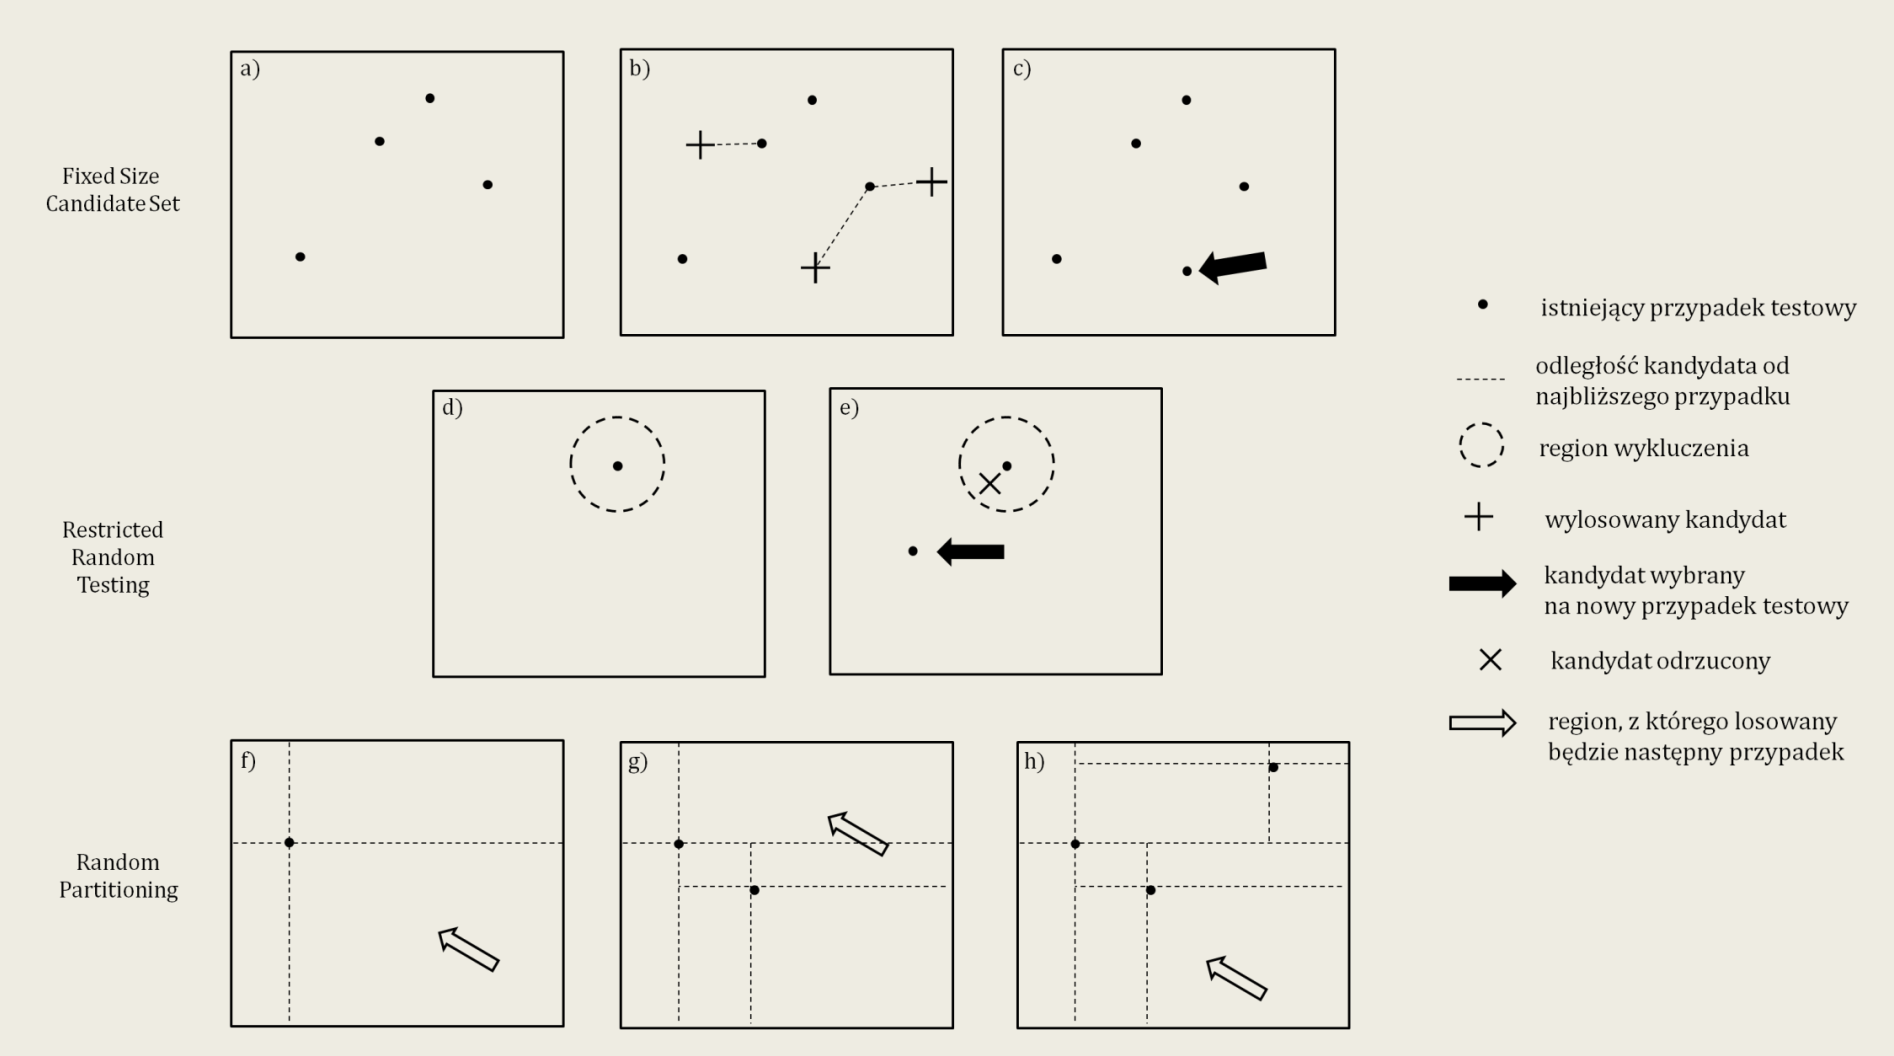
\includegraphics[width=\linewidth]{losowe.png}
    \end{figure}

    \subsubsection{Testowanie oparte na use-case'ach}
    \begin{itemize}
        \item przypadek użycia opisuje interakcję użytkownika z systemem
        \item zwykle wysokopoziomowy, w postaci przepływu „end-to-end”
        \item testowanie oparte na przypadkach użycia sprawdza poprawność
        działania systemu dla przepływów: głównego i alternatywnych
    \end{itemize}

    \textbf{Generowanie przypadków użycia:}
    \begin{enumerate}
        \item Dla każdego przypadku użycia wygeneruj pełny zbiór scenariuszy
        \item Dla każdego scenariusza zidentyfikuj przynajmniej 1 przypadek testowy i warunki
        umożliwiające jego wykonanie
        \item Dla każdego przypadku testowego zidentyfikuj dane, dla których można przeprowadzić test
    \end{enumerate}


    \subsubsection{Testowanie CRUD}

    \begin{itemize}
        \item CRUD = Create, Read, Update, Delete
        \item metoda testowania cyklu życia danych (encji)
        \item cykl życia reprezentowany przy pomocy tzw. macierzy CRUD
        \begin{itemize}
            \item wiersze = funkcje, kolumny = encje, przecięcie = operacja
            \item dla każdej funkcji sprawdzamy które encje są wykorzystywane
            \item a następnie, które akcje (C, R, U, D) są na nich przeprowadzane
        \end{itemize}
        \item dwa rodzaje testów
        \begin{itemize}
            \item sprawdzanie kompletności (statyczny)
            \begin{itemize}
                \item sprawdzenie, czy dla każdej encji występują wszystkie 4 operacje
                \item brak jakiejś akcji niekoniecznie oznacza błąd w systemie, ale powód tego braku powinien zostać wyjaśniony
            \end{itemize}
            \item sprawdzanie spójności (dynamiczny)
            \begin{itemize}
                \item sprawdza integrację różnych funkcji
                \item przypadki testowe konstruujemy zadając cały cykl życia encji:
                \item każdy przypadek testowy zaczyna się od C i przechodzi do
                wszystkich możliwych U, kończąc na D; jeśli jest więcej możliwości
                C i D, tworzy się dodatkowe przypadki
                \item po każdej akcji (C, U, D) występuje jedno lub kilka R – to sprawdza,
                czy encja została poprawnie przetworzona i jest użyteczna dla innych funkcji
                \item dla każdej encji, wszystkie wystąpienia akcji (C, R, U i D) we
                wszystkich funkcjach powinny zostać pokryte przez przypadki testowe
            \end{itemize}
        \end{itemize}
    \end{itemize}


\end{document}
